\section{Introduction}\label{sec:spmv-intro}

The product of a sparse matrix and a dense vector (\textbf{SpMV}) is a key part of many codes from disparate areas. Numerically, it makes up the bulk of the High Performance Conjugate (HPCG) \cite{techbib:hpcg-snl-dongarra} code that has become an alternative to LINPACK for rating supercomputers.\footnote{http://www.hpcg-benchmark.org/} When the matrix operations are changed from product and add to a variety of other non-numeric functions that still form semirings, it becomes an essential part of many graph kernels \cite{bigdata:doi:10.1137/1.9780898719918}, and is a key function in the recently released GRAPHBLAS spec \cite{http://graphblas.org/index.php?title=Graph_BLAS_Forum}. There has even been a novel prototype hardware system built around such sparse operations \cite{techbib:song-hpec}.

\begin{figure}\begin{centering}
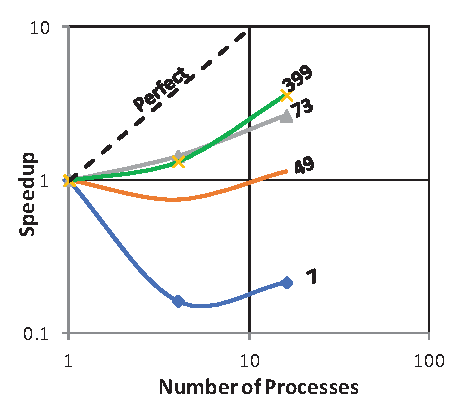
\includegraphics[scale=0.85]{../figures/spmv-bylina-speedup.eps}
\caption{Speedup from \cite{techbib:6933066} for 4 Sparse Martices.}
\label{fig:spmv-bylina-speedup}
\end{centering}\end{figure}

In particular, motivating the work presented here was an earlier study \cite{techbib:6933066} that looked at scaling of SpMV for a variety of matrices of varying sparsity from a well-known repository.\footnote{https://www.cise.ufl.edu/research/sparse/matrices/} What caught our interest was an observed significant dip in speedup (see Fig. \ref{fig:spmv-bylina-speedup} where the numbers on each line is the average non-zeros per row) that approached an order of magnitude  for the sparsest cases, and from which recovery was slow as the available compute resources increased. We have observed similar dips in other kernels and wanted to explore this phenomena more closely. 

Our specific goal was thus to duplicate the results, explore the cause of the dip, and extend the range of scaling, all as a precursor for developing better codes for these very sparse cases that would scale well to very large systems. However, in the process of performing this study, we found that the matrices used (all symmetric) were filed in the repository in a compressed lower form with only the lower diagonal half of non-zeroes stored, and that even though the matrices were discussed in \cite{techbib:6933066} in terms of their actual uncompressed sparsity, the computational results seemed to have used only this lower half, which approximately halved the effective sparsity, and distorted the distribution of non-zeroes.  The work here has used the full version of these matrices.

In organization, Section \ref{spmv-analytic} discusses the generic algorithm and then builds a simple model for estimating performance. Section \ref{sec:spmv-prior} discusses some other prior work. Section \ref{sec:implementation} discusses the code implemented here.Section \ref{sec:evaluation} evaluates the results. Section \ref{sec:conclude} concludes.

